\documentclass[12pt,letterpaper]{article}

% ============================================================================
% PACKAGES
% ============================================================================
\usepackage[utf8]{inputenc}
\usepackage[T1]{fontenc}
\usepackage{geometry}
\usepackage{amsmath,amssymb,amsthm}
\usepackage{graphicx}
\usepackage{booktabs}      % For professional tables (toprule, midrule, bottomrule)
\usepackage{siunitx}       % For aligned numeric columns
\usepackage{threeparttable} % For tidy notes under tables
\usepackage{longtable}     % For multi-page tables
\usepackage{multirow}      % For multi-row cells
\usepackage{array}         % For column formatting
\usepackage{float}      % For table/figure placement
\usepackage{hyperref}   % For links and references
\usepackage{natbib}     % For citations (adjust to your style)
\usepackage{setspace}   % For line spacing
\usepackage{appendix}   % For appendices
\usepackage{xcolor}     % For colored text
\usepackage{fancyhdr}   % For headers/footers
\usepackage{titlesec}   % For custom section formatting

% ============================================================================
% PAGE SETUP
% ============================================================================
\geometry{
    left=1in,
    right=1in,
    top=1in,
    bottom=1in,
    headheight=14pt
}

% Line spacing: 1.5 for draft, 2.0 for final submission (check requirements)
\onehalfspacing

% ============================================================================
% SIUNITX CONFIGURATION (for aligned numeric columns in tables)
% ============================================================================
\sisetup{
    table-number-alignment = center,
    group-digits = integer,
    group-minimum-digits = 4,
    table-format = 2.2,  % Default: 2 digits before, 2 after decimal
}

% ============================================================================
% HYPERREF SETUP
% ============================================================================
\hypersetup{
    colorlinks=true,
    linkcolor=blue,
    citecolor=blue,
    urlcolor=blue,
    pdftitle={CNN Stock Prediction and FOMC Events},
    pdfauthor={Your Name}
}

% ============================================================================
% CUSTOM COMMANDS
% ============================================================================
% Statistical significance stars (for use in tables)
% Usage: $^{*}$, $^{**}$, $^{***}$ for 10%, 5%, 1% significance
\newcommand{\stars}[1]{%
    \ifnum#1<1 $^{***}$%
    \else\ifnum#1<5 $^{**}$%
    \else\ifnum#1<10 $^{*}$%
    \fi\fi\fi%
}

% Table notes (use threeparttable for better formatting)
\newcommand{\tablenote}[1]{\textit{Notes:} #1}

% ============================================================================
% TITLE PAGE
% ============================================================================
\title{Convolutional Neural Networks for Stock Return Prediction:\\
       Evidence from FOMC Announcements}
\author{Your Name\\
        Your University\\
        \texttt{your.email@university.edu}}
\date{\today}

% ============================================================================
% DOCUMENT
% ============================================================================
\begin{document}

% Title page
\maketitle
\thispagestyle{empty}
\newpage

% Abstract
\begin{abstract}
% ABSTRACT
% Replace this with your actual abstract content

This thesis examines the predictive power of convolutional neural networks (CNNs) for stock returns, with a particular focus on Federal Open Market Committee (FOMC) announcement days. I replicate the CNN-based prediction methodology of Jiang et al. (2023) and extend it to analyze cross-sectional return predictability during high-information macro events. Using a sample of 22,480 U.S. stocks from 2001-2024, I find that CNN predictions generate economically significant returns: equal-weighted high-minus-low portfolios earn 70.74\% annually with a Sharpe ratio of 5.60, while value-weighted portfolios earn 22.69\% annually. 

The main contribution is an event study of 217 FOMC meetings, which reveals significant cross-sectional predictability on announcement days (0.21\%, t=2.95, p$<$0.01) and in intermediate windows (0.35\%, t=2.24, p$<$0.05). However, when compared to matched non-FOMC days, FOMC periods show uniformly lower predictability across all horizons (differences of -0.49\% to -0.87\%, all t$>$4, p$<$0.001). This pattern supports the hypothesis that heightened market attention during macro events increases efficiency and compresses exploitable cross-sectional patterns, consistent with Hirshleifer and Sheng (2021). 

The predictability is concentrated in small-cap stocks (equal-weighted returns are 3-10× larger than value-weighted), suggesting that limited attention and limited arbitrage are key mechanisms. These findings demonstrate that machine learning predictability is state-dependent and varies with the information environment, providing new evidence on the interaction between attention, efficiency, and cross-sectional return predictability.


\end{abstract}

\newpage

% Table of Contents
\tableofcontents
\newpage

% List of Figures
\listoffigures
\newpage

% List of Tables
\listoftables
\newpage

% ============================================================================
% MAIN SECTIONS
% ============================================================================

% Introduction
\section{Introduction}
% INTRODUCTION
% TODO: Write your introduction here
% Use the content from your markdown files as a starting point

\subsection{Research Question}

\subsection{Motivation}

\subsection{Contributions}

\subsection{Structure of the Thesis}



% Literature Review
\section{Literature Review}
% LITERATURE REVIEW
% TODO: Write your literature review here
% Reference: chatgpt_prompts/CHATGPT_PROMPT_FOR_INTRO_LIT_REWRITE.md

\subsection{Machine Learning in Finance}

\subsection{Cross-Sectional Return Predictability}

\subsection{Event Studies and FOMC Announcements}

\subsection{Attention and Market Efficiency}



% Methodology
\section{Methodology}
% METHODOLOGY
% TODO: Write your methodology here
% Reference: chatgpt_prompts/CHATGPT_PROMPT_FOR_METHODOLOGY_FINAL.md
% Reference: METHODOLOGY_EXPLAINED_STEP_BY_STEP.md

\subsection{CNN Architecture}

\subsection{Data Preprocessing}

\subsection{Portfolio Construction}

\subsection{FOMC Event Study Design}

\subsection{Statistical Tests}



% Data
\section{Data}
% DATA SECTION
% This section describes your dataset

\subsection{Sample Period}

\subsection{Stock Universe}

\subsection{FOMC Dates}

\subsection{Summary Statistics}

% Include Table 1 here
\input{../thesis_output/tables/table1_sample_statistics.tex}



% Results
\section{Results}
% RESULTS SECTION
% TODO: Write your results here
% Reference: chatgpt_prompts/CHATGPT_PROMPT_FOR_RESULTS_FINAL.md

\subsection{Baseline CNN Replication}

% Table 3: EW Portfolio Performance
\input{../thesis_output/tables/table3_portfolio_ew.tex}

% Table 4: VW Portfolio Performance
\input{../thesis_output/tables/table4_portfolio_vw.tex}

% Figure 2: Decile Performance
\begin{figure}[H]
\centering
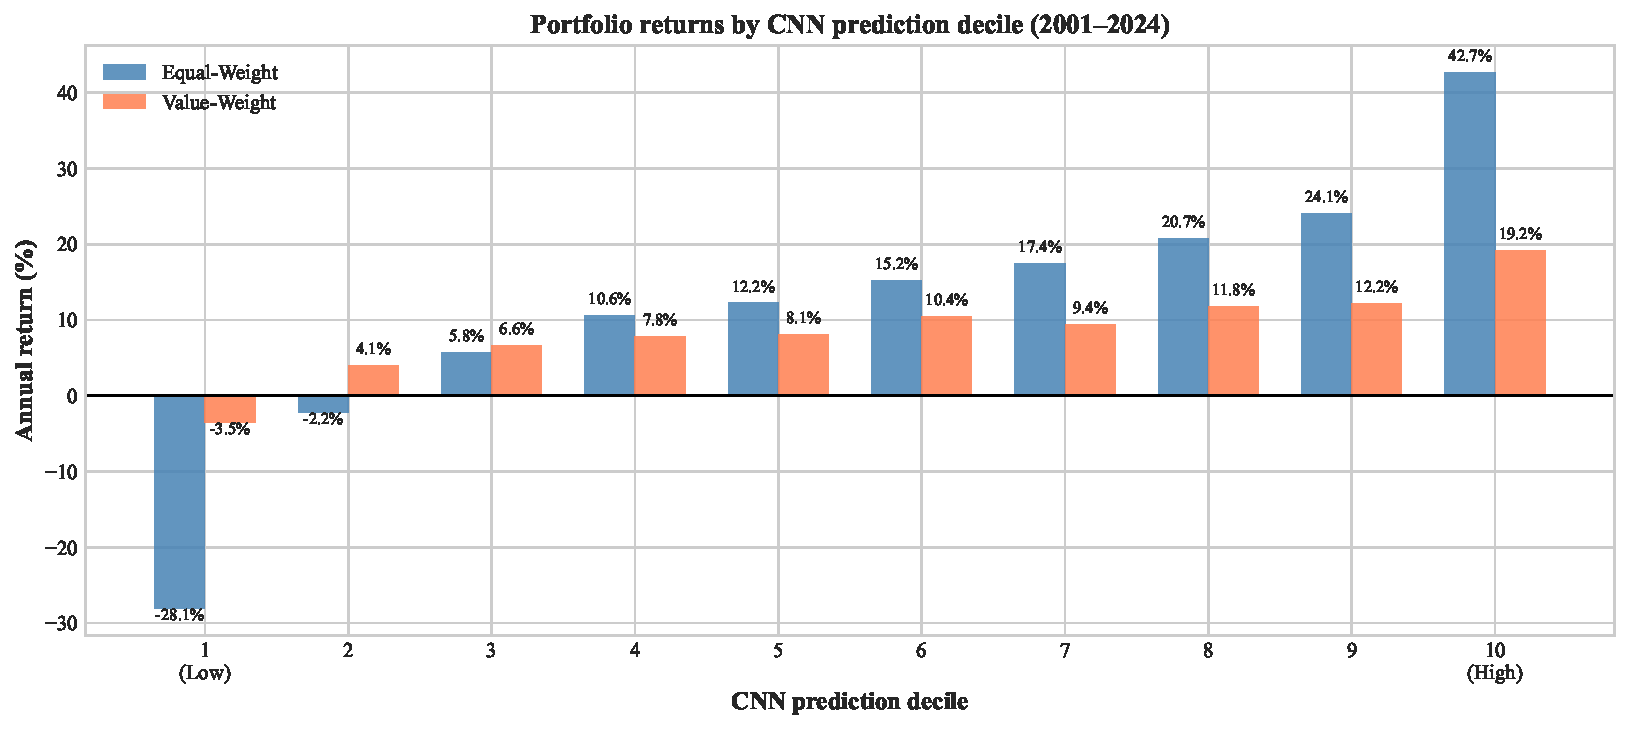
\includegraphics[width=0.8\textwidth]{../thesis_output/figures/figure2_decile_performance.pdf}
\caption{Decile Portfolio Performance}
\label{fig:decile_performance}
\end{figure}

\subsection{Horizon Evaluation}

% Table 2: Horizon Evaluation
\input{../thesis_output/tables/table2_horizon_evaluation.tex}

% Figure 3: Horizon Evaluation
\begin{figure}[H]
\centering
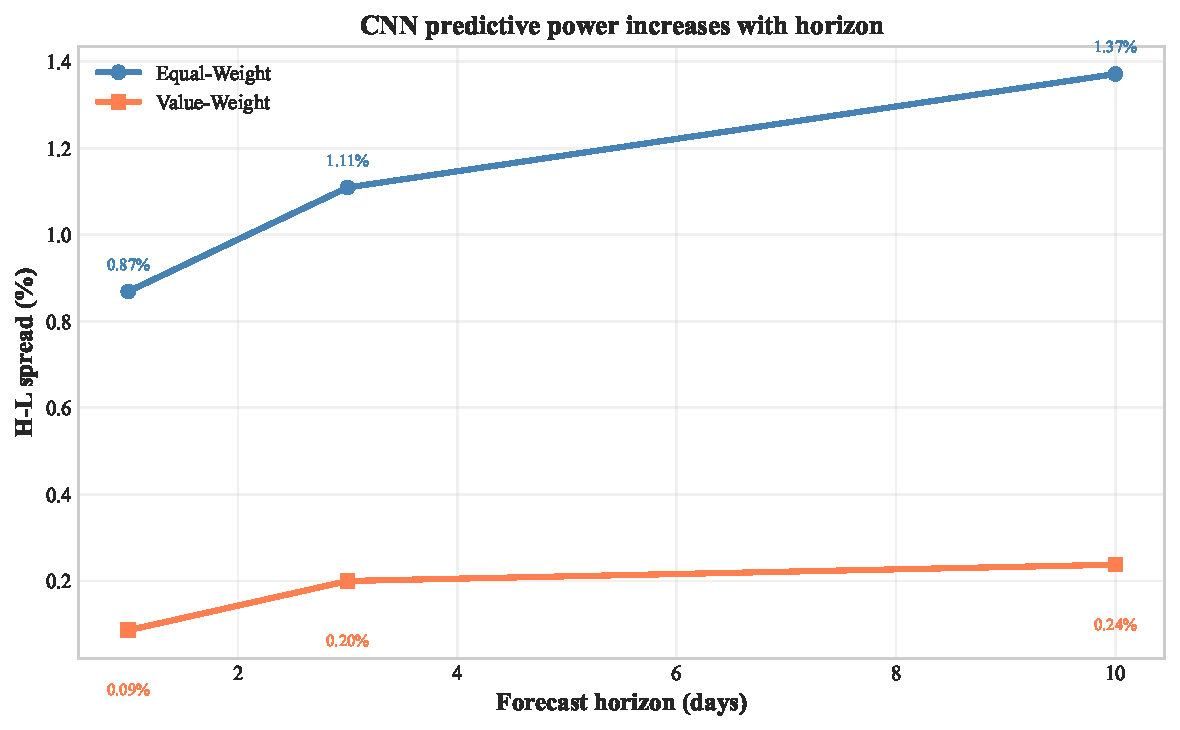
\includegraphics[width=0.8\textwidth]{../thesis_output/figures/figure3_horizon_evaluation.pdf}
\caption{Horizon Evaluation}
\label{fig:horizon_eval}
\end{figure}

\subsection{FOMC Event Study}

% Table 5: FOMC Event Study
\input{../thesis_output/tables/table5_fomc_event_study.tex}

% Table 5a: Announcement Day
\input{../thesis_output/tables/table5a_announcement_day.tex}

% Figure 4: FOMC Results
\begin{figure}[H]
\centering
\includegraphics[width=0.8\textwidth]{../thesis_output/figures/figure4_fomc_results.pdf}
\caption{FOMC Event Study Results}
\label{fig:fomc_results}
\end{figure}

\subsection{FOMC vs Matched Non-FOMC Comparison}

% Table 6: FOMC vs Matched
\input{../thesis_output/tables/table6_fomc_vs_matched.tex}

% Figure 5: FOMC vs Matched
\begin{figure}[H]
\centering
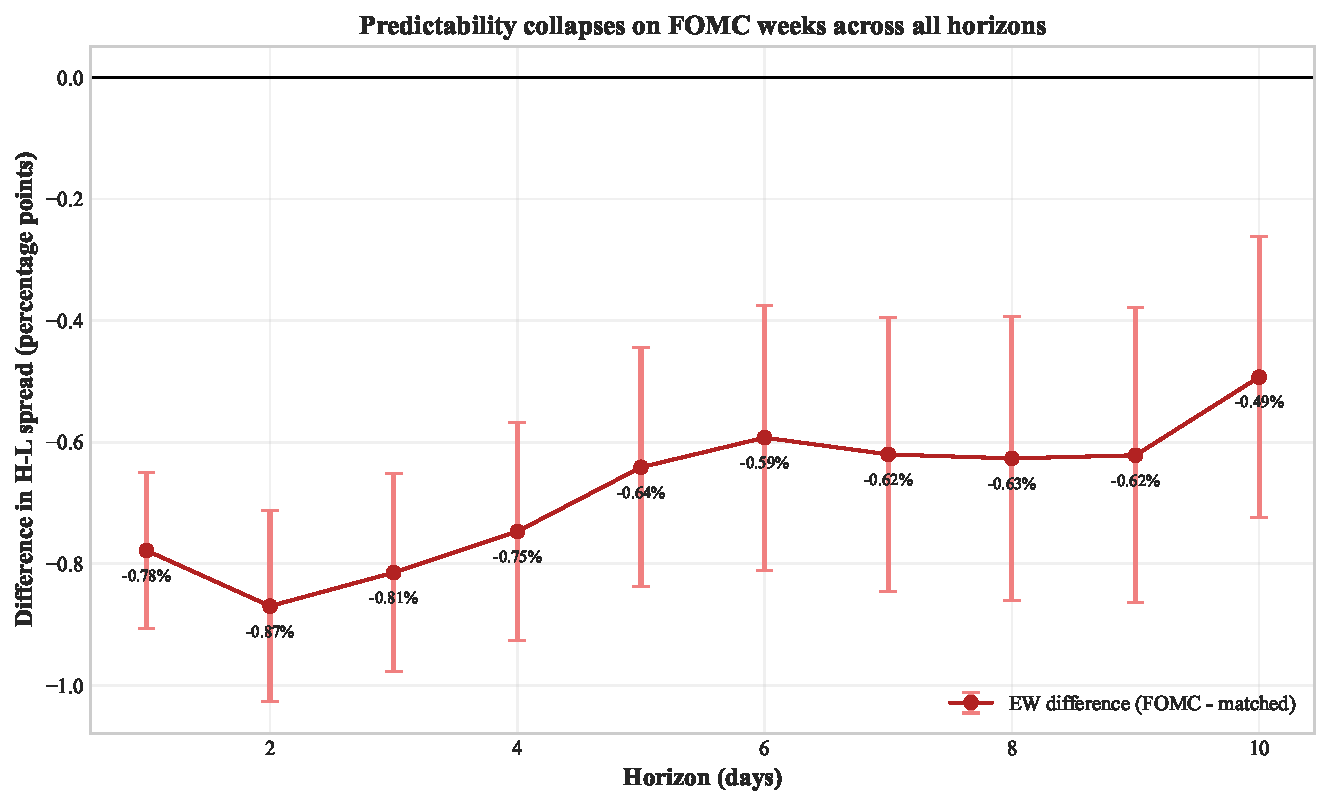
\includegraphics[width=0.8\textwidth]{../thesis_output/figures/figure5_fomc_vs_matched.pdf}
\caption{FOMC vs Matched Non-FOMC Comparison}
\label{fig:fomc_vs_matched}
\end{figure}

\subsection{Equal-Weighted vs Value-Weighted Analysis}

% Table 6: EW vs VW Comparison
\input{../thesis_output/tables/table6_ew_vw_comparison.tex}

% Table 7: EW vs VW Summary
\input{../thesis_output/tables/table7_ew_vs_vw_summary.tex}

% Figure 5: EW vs VW
\begin{figure}[H]
\centering
\includegraphics[width=0.8\textwidth]{../thesis_output/figures/figure5_ew_vw_comparison.pdf}
\caption{Equal-Weighted vs Value-Weighted Comparison}
\label{fig:ew_vw_comparison}
\end{figure}

\subsection{Size-Sorted Analysis}

% Table 8: Size-Sorted
\input{../thesis_output/tables/table8_size_sorted.tex}



% Discussion
\section{Discussion}
% DISCUSSION SECTION
% TODO: Write your discussion here
% Reference: chatgpt_prompts/CHATGPT_PROMPT_FOR_DISCUSSION_FINAL.md

\subsection{Interpretation of Main Findings}

\subsection{Attention-Based Efficiency Mechanism}

\subsection{Small-Cap Concentration}

\subsection{Limitations and Future Research}



% Conclusion
\section{Conclusion}
% CONCLUSION SECTION
% TODO: Write your conclusion here
% Reference: chatgpt_prompts/CHATGPT_PROMPT_FOR_CONCLUSION_FINAL.md

\subsection{Summary of Contributions}

\subsection{Implications}

\subsection{Future Directions}



% ============================================================================
% REFERENCES
% ============================================================================
\newpage
\bibliographystyle{aer}  % Adjust to your required style (aer, apalike, etc.)
\bibliography{references}  % Your .bib file

% ============================================================================
% APPENDICES
% ============================================================================
\newpage
\begin{appendices}
\section{Additional Tables}
% ADDITIONAL TABLES
% Include any supplementary tables here

% Table 7: Transaction Costs
\input{../../thesis_output/tables/table7_transaction_costs.tex}

% Table 9: FOMC Timeline
\begin{table}[ht]
\centering
\caption{Predictability around FOMC announcements. EW and VW high-minus-low spreads by window.}
\label{tab:fomc_timeline}
\begin{tabular}{lccccccc}
\toprule
Window & EW H-L (%) & EW t-stat & EW p-value & VW H-L (%) & VW t-stat & VW p-value & Events \\
\midrule
Pre-announcement (t-1 to t) & 0.21 & 2.95 & 0.00 & 0.05 & 0.66 & 0.51 & 216.00 \\
Announcement day (t) & 0.21 & 2.95 & 0.00 & 0.05 & 0.66 & 0.51 & 217.00 \\
Reaction (t+1) & 0.10 & 1.76 & 0.08 & 0.03 & 0.38 & 0.71 & 215.00 \\
Intermediate (t+4 to t+20) & 0.35 & 2.24 & 0.03 & -0.28 & -1.57 & 0.12 & 208.00 \\
\bottomrule
\end{tabular}
\end{table}


% Table 10: Decile Regimes
\begin{table}[ht]
\centering
\caption{Average decile returns on FOMC signal weeks versus matched control weeks (EW and VW). FOMC weeks: 216, matched weeks: 15.}
\label{tab:decile_regime}
\begin{tabular}{lcccccc}
\toprule
Decile & FOMC EW (%) & Matched EW (%) & Diff EW (%) & FOMC VW (%) & Matched VW (%) & Diff VW (%) \\
\midrule
Low (1) & -0.88 & -1.10 & 0.22 & -0.23 & -0.16 & -0.07 \\
Decile 2 & -0.27 & -0.59 & 0.32 & -0.09 & -1.13 & 1.05 \\
Decile 3 & -0.10 & -0.42 & 0.32 & 0.02 & -0.47 & 0.49 \\
Decile 4 & -0.01 & -0.38 & 0.37 & -0.02 & -0.73 & 0.71 \\
Decile 5 & 0.04 & -0.35 & 0.39 & 0.01 & -0.92 & 0.94 \\
Decile 6 & 0.12 & -0.30 & 0.42 & 0.02 & -0.42 & 0.45 \\
Decile 7 & 0.18 & -0.58 & 0.75 & -0.02 & -0.68 & 0.65 \\
Decile 8 & 0.23 & -0.35 & 0.58 & 0.09 & -0.32 & 0.41 \\
Decile 9 & 0.33 & -0.18 & 0.51 & 0.02 & -0.23 & 0.25 \\
High (10) & 0.73 & 0.69 & 0.04 & 0.09 & -0.50 & 0.60 \\
H-L & 1.61 & 1.79 & -0.19 & 0.32 & -0.34 & 0.67 \\
\bottomrule
\end{tabular}
\end{table}




\section{Additional Figures}
% ADDITIONAL FIGURES
% Include any supplementary figures here

% Figure 1: FOMC Timeline
\begin{figure}[H]
\centering

\includegraphics[width=0.8\textwidth]{../../thesis_output/figures/figure1_fomc_timeline.pdf}
\caption{FOMC Timeline: No Overlap Proof}
\label{fig:fomc_timeline}
\end{figure}

% Figure 6: CNN Architecture
\begin{figure}[H]
\centering
\includegraphics[width=0.8\textwidth]{../../thesis_output/figures/figure6_cnn_architecture.pdf}
\caption{CNN Architecture}
\label{fig:cnn_architecture}
\end{figure}

% Figure 7: Cumulative Returns
\begin{figure}[H]
\centering
\includegraphics[width=0.8\textwidth]{../../thesis_output/figures/figure7_cumulative_returns.pdf}
\caption{Cumulative Portfolio Returns}
\label{fig:cumulative_returns}
\end{figure}

% Figure 8: Prediction Distribution
\begin{figure}[H]
\centering

\includegraphics[width=0.8\textwidth]{../../thesis_output/figures/figure8_prediction_distribution.pdf}
\caption{Prediction Distribution}
\label{fig:prediction_distribution}
\end{figure}



\section{Robustness Checks}
% ROBUSTNESS CHECKS
% Document any robustness checks here

\subsection{Outlier Analysis}

\subsection{Winsorization}

\subsection{Alternative Specifications}

\subsection{Sample Period Sensitivity}


\end{appendices}

\end{document}

